\documentclass{beamer}
\usepackage[utf8]{inputenc}
\usepackage[T1]{fontenc}
\usepackage[french]{babel}

\usepackage[export]{adjustbox}
\usepackage{array}
\usepackage{color, colortbl}

\usepackage{graphicx}

\usetheme{JuanLesPins}
\setbeamercolor{structure}{fg=arkred}, bg=arkred}

% colors
\definecolor{gray73}{gray}{0.73}
\definecolor{arkred}{rgb}{0.592, 0.145, 0.168}
\definecolor{arkbrown}{rgb}{0.239,0.235,0.204}

\graphicspath{{../images/}}

\title{Rapport de stage \\Master 2 -- Fiabilité et Sécurité Informatique}
\subtitle{Conception \&  d\'eveloppement syst\`eme de backup chiffr\'e et
incr\'emental en C/C++}
\author{Ludovic Lubeigt}
\institute{Aix-Marseille University}
\date{18 septembre 2015}

\AtBeginSubsection[]
{
  \begin{frame}
  \frametitle{Sommaire}
  \tableofcontents[currentsection, currentsubsection, hideothersubsection]
  \end{frame} 
}

\AtBeginSection[]
{
  \begin{frame}
   \frametitle{Sommaire}
   \tableofcontents[currentsection, hideothersubsection]
  \end{frame}
}

\begin{document}
\begin{frame}
 \titlepage
\end{frame}

\begin{frame}
 \frametitle{Sommaire}
 \tableofcontents
\end{frame}

\section{Arksens}
\subsection{Pr\'esentation de l'entreprise}
\begin{frame}
 \frametitle{Arksens}
 \framesubtitle{Pr\'esentation de l'entreprise}
 \begin{minipage}{0.49\textwidth}
  \begin{itemize}
    \item Une pr\'esence sur 3 continents
    \item 6 produits
    \item 3 offres clouds
  \end{itemize}
 \end{minipage}
 \begin{minipage}{0.49\textwidth}
  \begin{figure}[h!]
    \centering
    \includegraphics[scale=0.15]{map_arksens.png}
    \caption{\label{mapArksens} O\`u trouver Arksens}
  \end{figure}
 \end{minipage}
\end{frame}

\begin{frame}
  \frametitle{Arksens}
  \framesubtitle{Les produits et Services}
  \begin{table}[h!]
  \centering
  \def\arraystretch{1.5}
  \setlength{\fboxsep}{13pt} % padding
  \setlength{\fboxrule}{0pt} % frame
  \begin{tabular}{cc}
    \arrayrulecolor{gray73}
    \includegraphics[width=3cm, fbox]{produits/mail.png} & 
    \includegraphics[width=3cm, fbox]{produits/whisper.png}\\
    \hline
    \includegraphics[width=3cm, fbox]{produits/backup.png} &
    \includegraphics[width=3cm, fbox]{produits/gateway.png}\\
    \hline
    \includegraphics[width=3cm, fbox]{produits/endpoint.png} &
    \includegraphics[width=3cm, fbox]{produits/nomad.png}\\
  \end{tabular}
  \caption{\label{tabProduits} Produits et solutions par \textit{Arksens}}
\end{table}
\end{frame}

\subsection{\^Ile Maurice}
\begin{frame}
  \frametitle{Arksens}
  \framesubtitle{\^Ile Maurice}
  \begin{minipage}{0.49\linewidth}
    \begin{itemize}
     \item Recherche et d\'eveloppement
     \item Jusqu'\`a 8 employ\'es + des commerciaux et le PDG
     \item Importante restructuration
    \end{itemize}
  \end{minipage}
  \begin{minipage}{0.49\linewidth}
    \begin{figure}[h!]
      \centering
      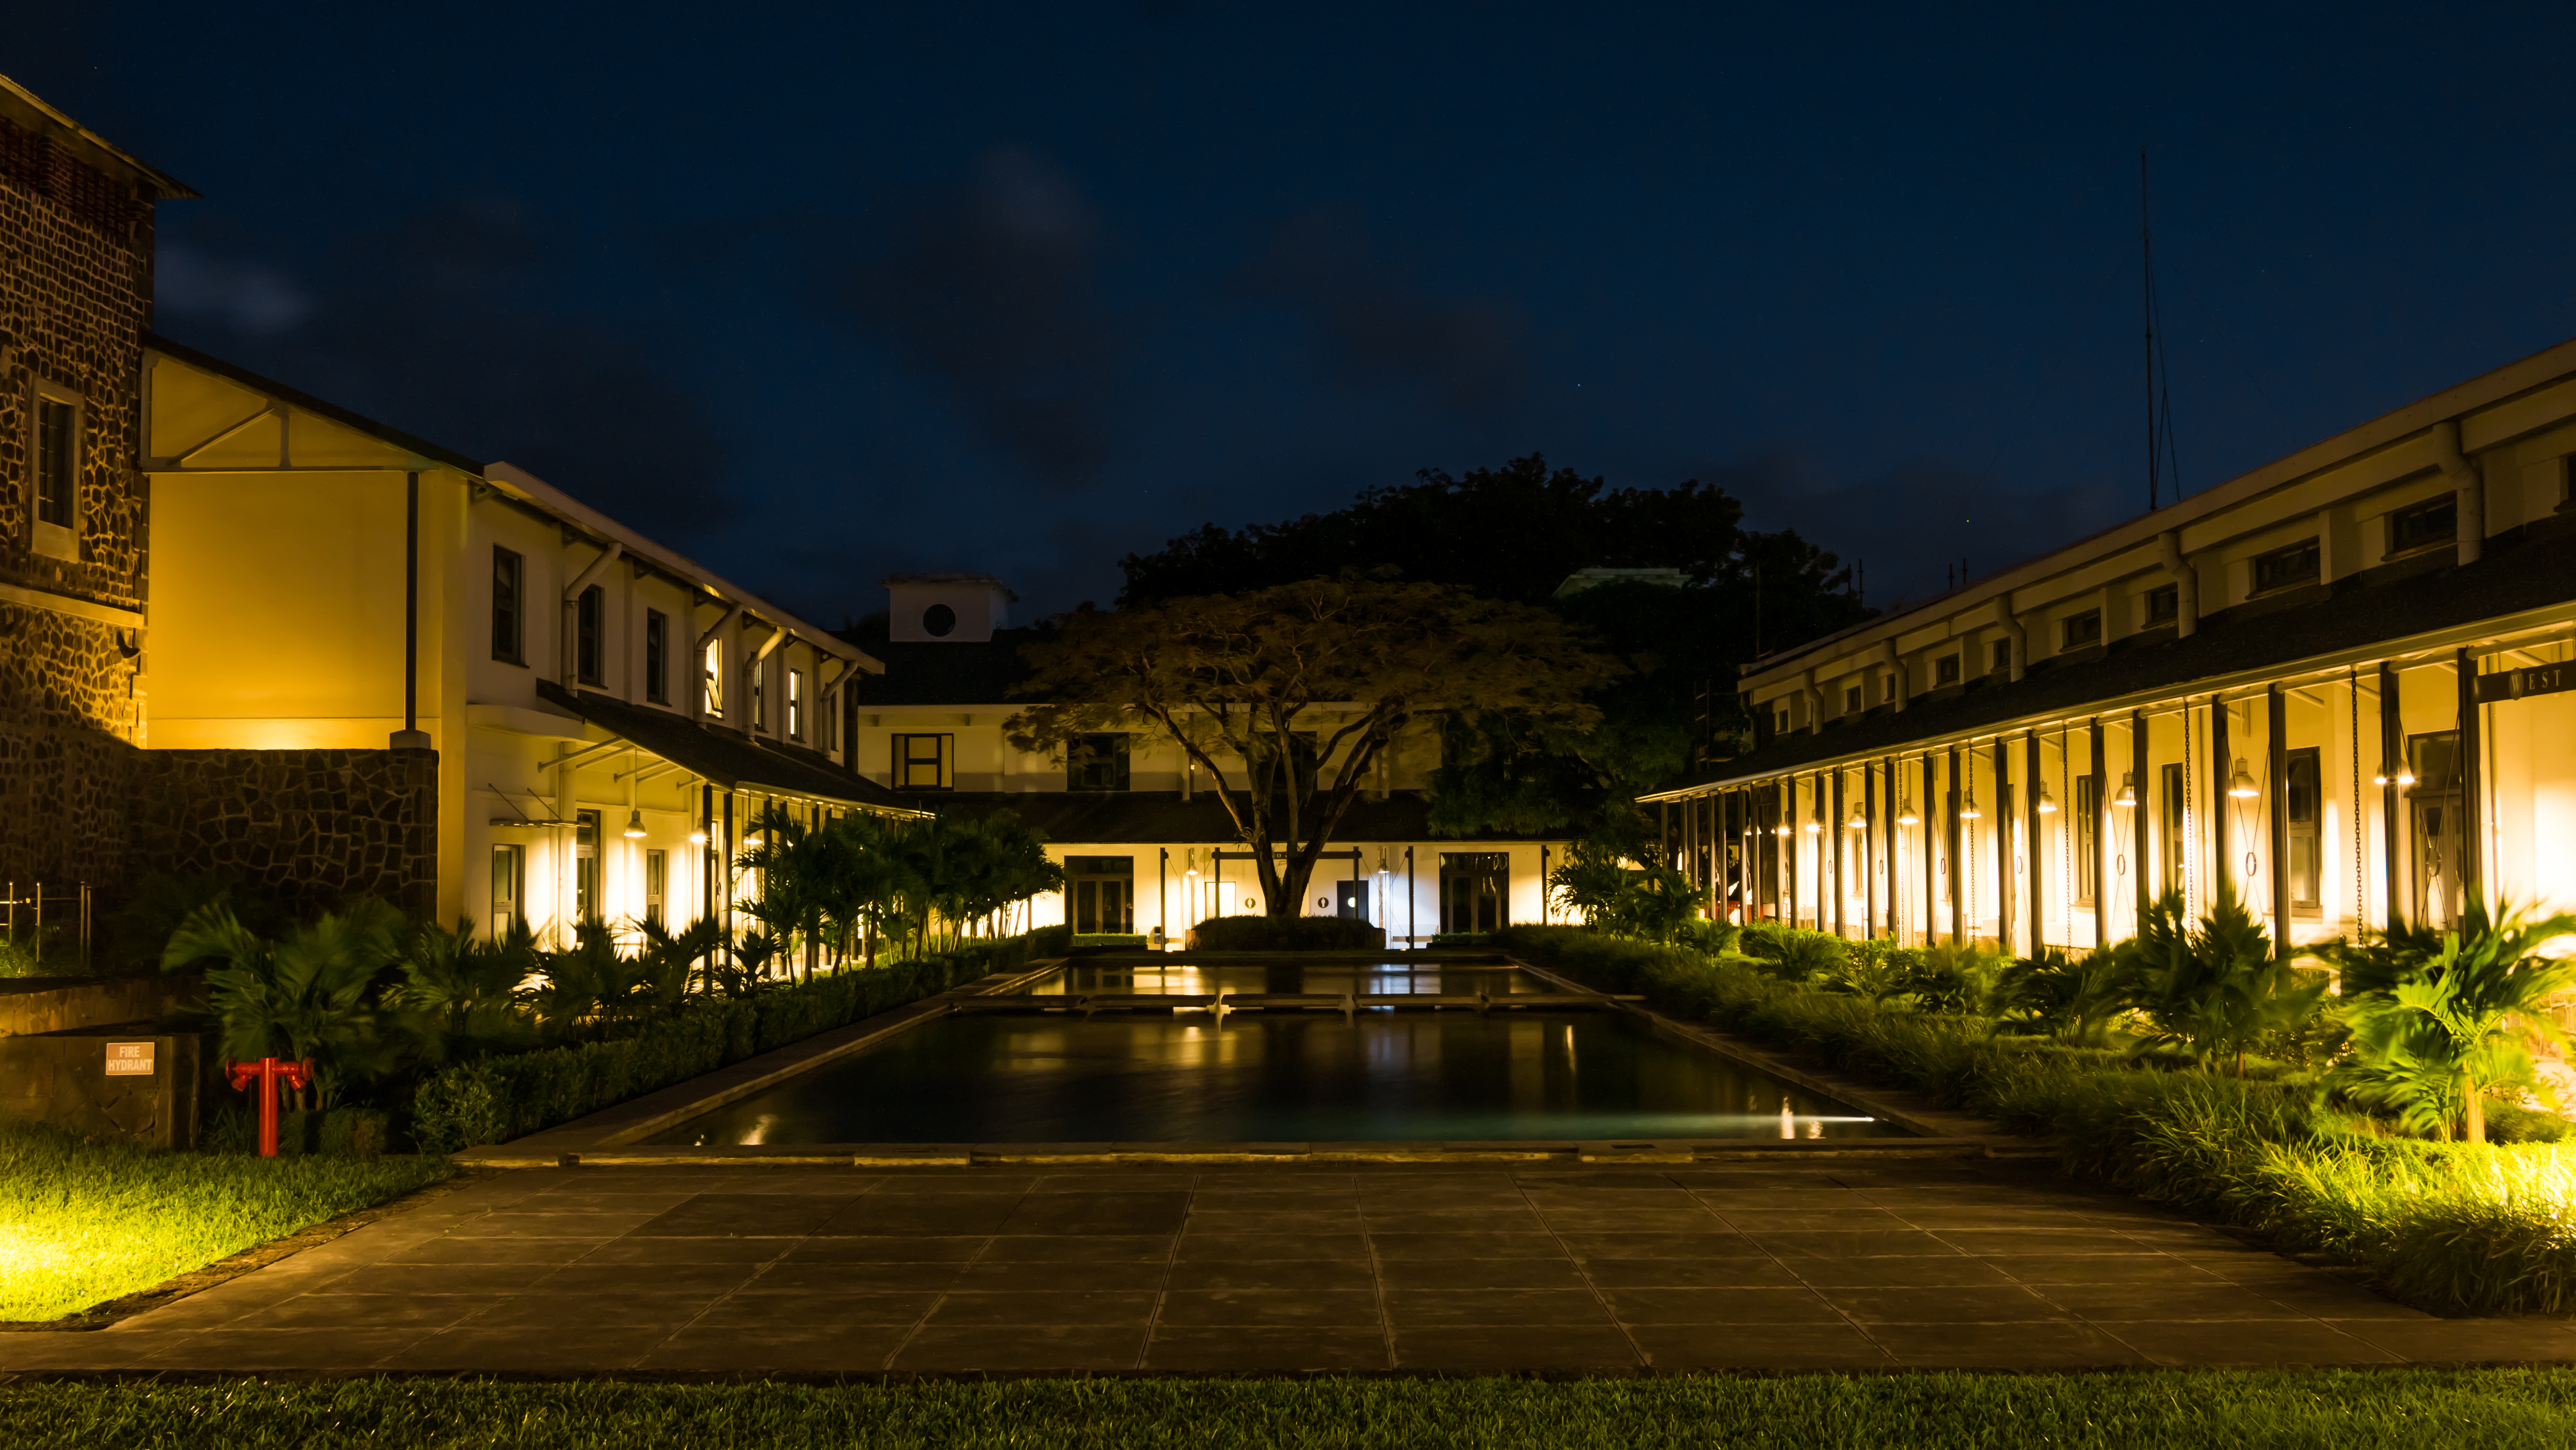
\includegraphics[scale=0.23]{beau_plan_soir.jpg}
      \caption{\label{beauPlan} Beau Plan Business Park}
    \end{figure}
  \end{minipage}

\end{frame}

\section{Conclusion}
\begin{frame}
 \frametitle{Conclusion}
 \begin{itemize}
  \item TODO
  \item TODO
  \item TODO
 \end{itemize}
\end{frame}

\section*{Questions}
\begin{frame}
\frametitle{Questions}
Questions ?
\end{frame}

\section*{Remerciements}
\begin{frame}
 \frametitle{Remerciements}
 Merci de votre attention !
\end{frame}


\end{document}